\section{Study Settings}

\begin{figure*}[ht]
  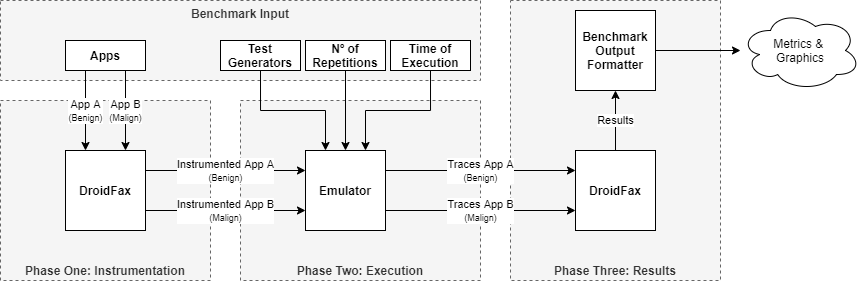
\includegraphics[width=1\textwidth]{images/benchmark3.png}
  \label{benchArq}
  \caption{Benchmark architecture}
  \label{fig:benchArq}
\end{figure*}

In this section, we present the setting of our study, whose main goal is to perform a non-exact replication of the work of Bao et al. and understand the implications of static analysis algorithms in his results. We also investigate how static analysis can improve the performance of mining sandboxes, in the task of identifying malicious behaviors.

To achieve this general goal, we answer the following research questions. 

\begin{enumerate}[(RQ1)]
\item What benefits of using a hybrid approach, which combines static and dynamic analysis, for mining sandboxes ?
\item What is the effective performance of each tool in terms of the number of detected malware ?
\item What is the impact of static analysis on benchmark results ?
\end{enumerate}

To answer the research questions above, we conduct two experiments using a benchmark solution called droidXP \cite{DBLP:conf/scam/CostaMCMVBC20}. This benchmark help us to reproduce Bao et al. work on mining sandboxes, allowing integrate different test case tools, define your execution time, and the number of experiment repetitions. The (Figure \ref{fig:benchArq}) show all details of the benchmark architecture used in our experiments. The benchmark runs these tools in benign apps and, based on resources sensitives access in this execution, we build their sandbox.

At both experiments, we employed the same dataset, 98 pair of real-world apps (B/M), shared by the AndroZoo \cite{DBLP:conf/msr/AllixBKT16} group. We executed each app in each one of the five test generator tool, selected for our study, for three minutes, and for just one time. The droidXP benchmark relies on DroidFax, the same tool used by Bao et al. in your study. Droidfax instrumented Android apps and collected relevant information about their execution (using the test case generation tools). It collects the set of sensitive APIs accessed during test execution, and during a static analysis at each code apps. Based on these sensitive APIs, that will compose the sandbox, we investigate the capacity to detect malicious behaviors in the corresponding malign app by the tool under analysis, together with the DroidFax static analysis. (Figure \ref{fig:setup}) show this experiment setup. We detail the procedures of each study in what follows.

\begin{figure}[h]
  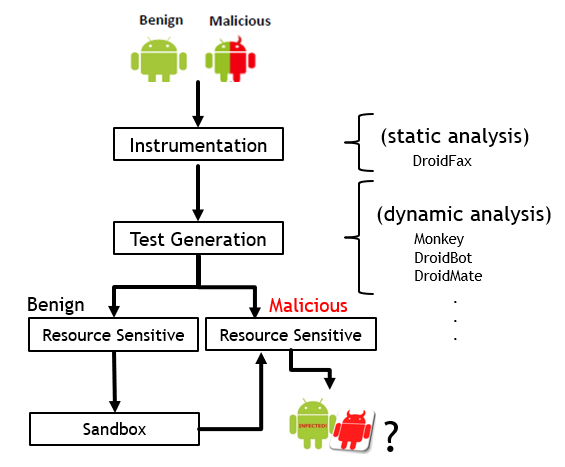
\includegraphics[width=0.45\textwidth]{images/setup.png}
  \label{Experiment setup}
  \caption{Experiment setup}
  \label{fig:setup}
\end{figure}

\subsection{First Study: hybrid proposal}

In the first experiment, we executed the benchmark using the droidXP default configuration, that is, combining static and dynamic analysis while collecting the accessed sensitive APIs, a hybrid approach. To generate inputs to apps, we investigate five popular test case generation tools, one from industry (Monkey \cite{Monkey}) and four from academia (Droidbot \cite{DBLP:conf/icse/LiYGC17}, Humanoid \cite{DBLP:conf/kbse/LiY0C19}, DroidMate \cite{DBLP:conf/icse/JamrozikZ16} and ``Joke" tool). This last is a fake tool that simulates a tool that does nothing during the benchmark execution. Using this tool, the results of the dynamic analysis are not considered and we can compute the results with only the static analysis, performed by the benchmark droidXP. So, we used this experiment to answer the research questions (RQ1) and (RQ3), since the ``Joke" tool result presented the real impact of static analysis on benchmark, assuming that our fake tools, do not performs dynamic analysis.

\subsection{Second Study: Dynamic analysis proposal}

In this second experiment, we used an option of the benchmark that disables the static analysis performed by DroidFax. With this new configuration, we conduct our second study, with the same dataset apps from the first, the same execution time, and the same test case generation tools, including our ``Joke" tool. With the results, it was possible to compute the real aid portion of the dynamic analysis in the malware detection of each test generation tool, since the results, was computed without the static analysis DroidFax influence. We used this experiment to answer the research questions (RQ2) and also complements (RQ3), since it is expected that our fake tool will not be able to detect malware with this benchmark configuration, considering that it depends solely the DroidFax static analysis for this task.







